\documentclass[tikz]{standalone}
% \documentclass[tikz,convert={convertexe={convert_magick.exe}}]{standalone}

\usepackage{tikz}
\usepackage{xcolor}
\usetikzlibrary{calc}
\usetikzlibrary{arrows.meta}
\usetikzlibrary{trees}

\begin{document}

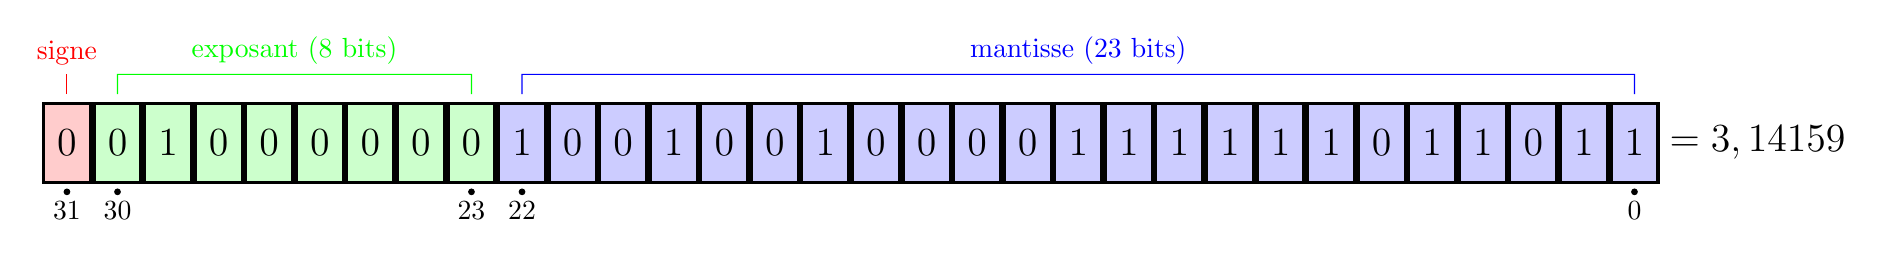
\begin{tikzpicture}

\tikzset{
    box/.style = {
    minimum height=1cm,
    minimum width = 0.6cm
    }
}

\tikzstyle{signe}=[draw, very thick, fill=red!20!white, box]
\tikzstyle{exposant}=[draw, very thick, fill=green!20!white, box]
\tikzstyle{mantisse}=[draw, very thick, fill=blue!20!white, box]

\matrix [column sep=0cm]
{
\node (f-31) [signe] {\Large 0}; 

& \node (f-30) [exposant] {\Large 0}; 
& \node (f-29) [exposant] {\Large 1}; 
& \node (f-28) [exposant] {\Large 0}; 
& \node (f-27) [exposant] {\Large 0}; 
& \node (f-26) [exposant] {\Large 0}; 
& \node (f-25) [exposant] {\Large 0}; 
& \node (f-24) [exposant] {\Large 0}; 
& \node (f-23) [exposant] {\Large 0}; 

& \node (f-22) [mantisse] {\Large 1}; 
& \node (f-21) [mantisse] {\Large 0}; 
& \node (f-20) [mantisse] {\Large 0}; 
& \node (f-19) [mantisse] {\Large 1}; 
& \node (f-18) [mantisse] {\Large 0}; 
& \node (f-17) [mantisse] {\Large 0}; 
& \node (f-16) [mantisse] {\Large 1}; 
& \node (f-15) [mantisse] {\Large 0};
& \node (f-14) [mantisse] {\Large 0};
& \node (f-13) [mantisse] {\Large 0};
& \node (f-12) [mantisse] {\Large 0};
& \node (f-11) [mantisse] {\Large 1};
& \node (f-10) [mantisse] {\Large 1};
& \node (f-9) [mantisse] {\Large 1};
& \node (f-8) [mantisse] {\Large 1};
& \node (f-7) [mantisse] {\Large 1};
& \node (f-6) [mantisse] {\Large 1};
& \node (f-5) [mantisse] {\Large 0};
& \node (f-4) [mantisse] {\Large 1};
& \node (f-3) [mantisse] {\Large 1};
& \node (f-2) [mantisse] {\Large 0};
& \node (f-1) [mantisse] {\Large 1};
& \node (f-0) [mantisse] {\Large 1};  
\\
};

\draw[red] ([shift=({0,0.1cm})]f-31.north)--++(0,0.25) node[above] {signe};

\draw[green] ([shift=({0,0.1cm})]f-30.north)--++(0,0.25)--([shift=({0,0.35cm})]f-23.north) node[midway, above] {exposant (8 bits)} --++(0,-0.25);

\draw[blue] ([shift=({0,0.1cm})]f-22.north)--++(0,0.25)--([shift=({0,0.35cm})]f-0.north) node[midway, above] {mantisse (23 bits)} --++(0,-0.25);

\foreach \i in {0,22,23,30,31}{
    \draw[fill=black] ([shift=({0,-0.1cm})]f-\i.south) circle (1pt) node[below] {\i};
}

% \draw ([shift=({0,1cm})]f-16.north) node[above] {\Large $\pi$};

\draw ([shift=({0,0cm})]f-0.east) node[right] {\Large $= 3,14159$};

\end{tikzpicture}


%%%

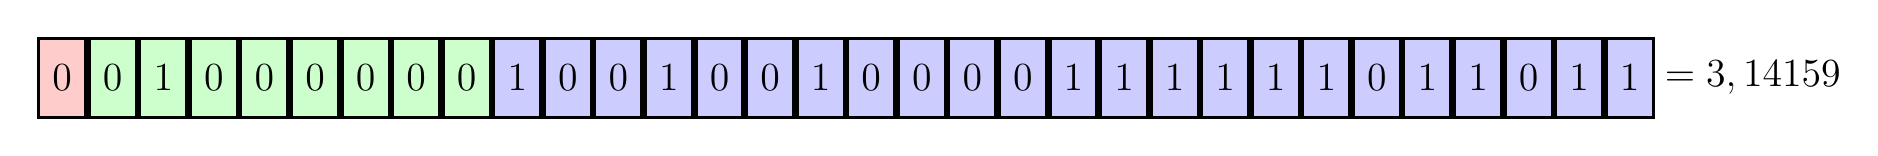
\begin{tikzpicture}

\tikzset{
    box/.style = {
    minimum height=1cm,
    minimum width = 0.6cm
    }
}

\tikzstyle{signe}=[draw, very thick, fill=red!20!white, box]
\tikzstyle{exposant}=[draw, very thick, fill=green!20!white, box]
\tikzstyle{mantisse}=[draw, very thick, fill=blue!20!white, box]

\matrix [column sep=0cm]
{
\node (f-31) [signe] {\Large 0}; 

& \node (f-30) [exposant] {\Large 0}; 
& \node (f-29) [exposant] {\Large 1}; 
& \node (f-28) [exposant] {\Large 0}; 
& \node (f-27) [exposant] {\Large 0}; 
& \node (f-26) [exposant] {\Large 0}; 
& \node (f-25) [exposant] {\Large 0}; 
& \node (f-24) [exposant] {\Large 0}; 
& \node (f-23) [exposant] {\Large 0}; 

& \node (f-22) [mantisse] {\Large 1}; 
& \node (f-21) [mantisse] {\Large 0}; 
& \node (f-20) [mantisse] {\Large 0}; 
& \node (f-19) [mantisse] {\Large 1}; 
& \node (f-18) [mantisse] {\Large 0}; 
& \node (f-17) [mantisse] {\Large 0}; 
& \node (f-16) [mantisse] {\Large 1}; 
& \node (f-15) [mantisse] {\Large 0};
& \node (f-14) [mantisse] {\Large 0};
& \node (f-13) [mantisse] {\Large 0};
& \node (f-12) [mantisse] {\Large 0};
& \node (f-11) [mantisse] {\Large 1};
& \node (f-10) [mantisse] {\Large 1};
& \node (f-9) [mantisse] {\Large 1};
& \node (f-8) [mantisse] {\Large 1};
& \node (f-7) [mantisse] {\Large 1};
& \node (f-6) [mantisse] {\Large 1};
& \node (f-5) [mantisse] {\Large 0};
& \node (f-4) [mantisse] {\Large 1};
& \node (f-3) [mantisse] {\Large 1};
& \node (f-2) [mantisse] {\Large 0};
& \node (f-1) [mantisse] {\Large 1};
& \node (f-0) [mantisse] {\Large 1};  
\\
};

\draw ([shift=({0,0cm})]f-0.east) node[right] {\Large $= 3,14159$};

% \draw ([shift=({0,0.5cm})]f-16.north) node[above] {\Large Représentation de $\pi$ comme un nombre en virgule flottante};

\end{tikzpicture}

%%%

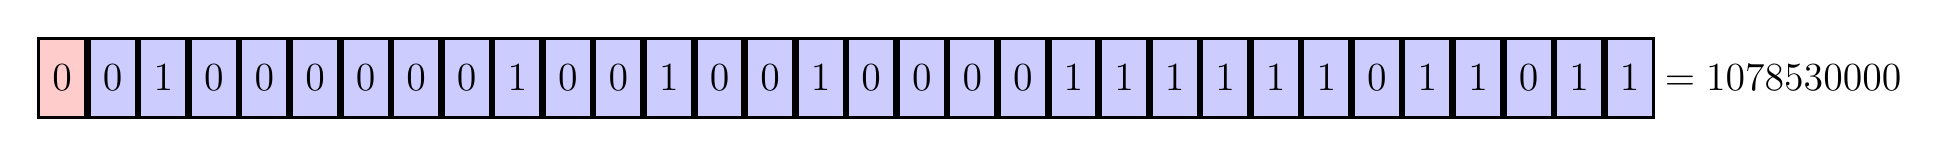
\begin{tikzpicture}

\tikzset{
    box/.style = {
    minimum height=1cm,
    minimum width = 0.6cm
    }
}

\tikzstyle{signe}=[draw, very thick, fill=red!20!white, box]
\tikzstyle{exposant}=[draw, very thick, fill=blue!20!white, box]
\tikzstyle{mantisse}=[draw, very thick, fill=blue!20!white, box]

\matrix [column sep=0cm]
{
\node (f-31) [signe] {\Large 0}; 

& \node (f-30) [exposant] {\Large 0}; 
& \node (f-29) [exposant] {\Large 1}; 
& \node (f-28) [exposant] {\Large 0}; 
& \node (f-27) [exposant] {\Large 0}; 
& \node (f-26) [exposant] {\Large 0}; 
& \node (f-25) [exposant] {\Large 0}; 
& \node (f-24) [exposant] {\Large 0}; 
& \node (f-23) [exposant] {\Large 0}; 

& \node (f-22) [mantisse] {\Large 1}; 
& \node (f-21) [mantisse] {\Large 0}; 
& \node (f-20) [mantisse] {\Large 0}; 
& \node (f-19) [mantisse] {\Large 1}; 
& \node (f-18) [mantisse] {\Large 0}; 
& \node (f-17) [mantisse] {\Large 0}; 
& \node (f-16) [mantisse] {\Large 1}; 
& \node (f-15) [mantisse] {\Large 0};
& \node (f-14) [mantisse] {\Large 0};
& \node (f-13) [mantisse] {\Large 0};
& \node (f-12) [mantisse] {\Large 0};
& \node (f-11) [mantisse] {\Large 1};
& \node (f-10) [mantisse] {\Large 1};
& \node (f-9) [mantisse] {\Large 1};
& \node (f-8) [mantisse] {\Large 1};
& \node (f-7) [mantisse] {\Large 1};
& \node (f-6) [mantisse] {\Large 1};
& \node (f-5) [mantisse] {\Large 0};
& \node (f-4) [mantisse] {\Large 1};
& \node (f-3) [mantisse] {\Large 1};
& \node (f-2) [mantisse] {\Large 0};
& \node (f-1) [mantisse] {\Large 1};
& \node (f-0) [mantisse] {\Large 1};  
\\
};

\draw ([shift=({0,0cm})]f-0.east) node[right] {\Large $= 1078530000$};

% \draw ([shift=({0,0.5cm})]f-16.north) node[above] {\Large Interprétation de la représentation de $\pi$ en virgule flottante comme un entier};

\end{tikzpicture}

%%%

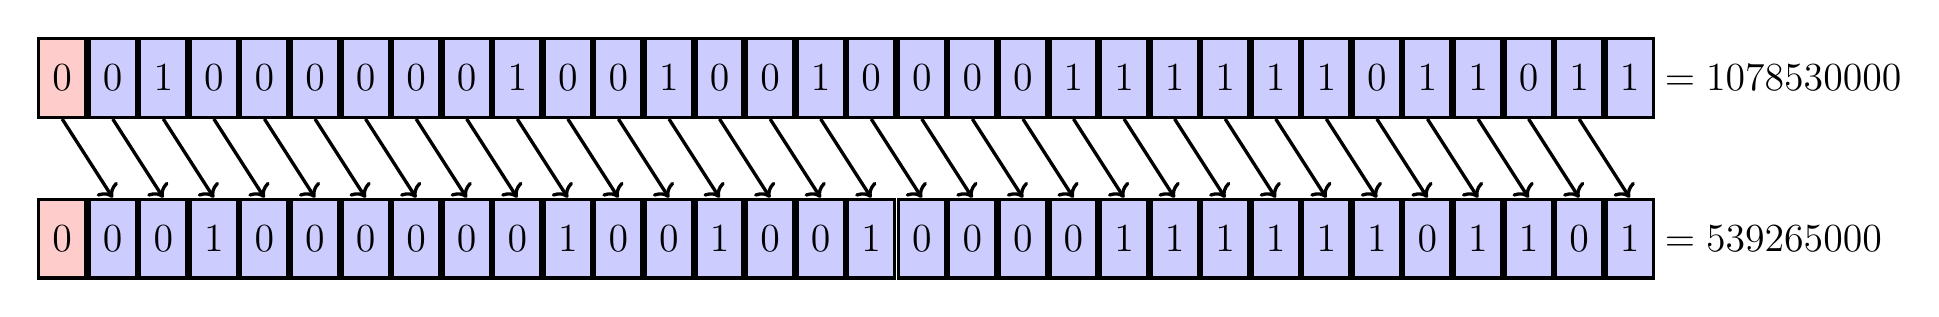
\begin{tikzpicture}

\tikzset{
    box/.style = {
    minimum height=1cm,
    minimum width = 0.6cm
    }
}

\tikzstyle{signe}=[draw, very thick, fill=red!20!white, box]
\tikzstyle{exposant}=[draw, very thick, fill=blue!20!white, box]
\tikzstyle{mantisse}=[draw, very thick, fill=blue!20!white, box]

\matrix [column sep=0cm, row sep=1cm]
{
\node (f-31) [signe] {\Large 0}; 

& \node (f-30) [exposant] {\Large 0}; 
& \node (f-29) [exposant] {\Large 1}; 
& \node (f-28) [exposant] {\Large 0}; 
& \node (f-27) [exposant] {\Large 0}; 
& \node (f-26) [exposant] {\Large 0}; 
& \node (f-25) [exposant] {\Large 0}; 
& \node (f-24) [exposant] {\Large 0}; 
& \node (f-23) [exposant] {\Large 0}; 

& \node (f-22) [mantisse] {\Large 1}; 
& \node (f-21) [mantisse] {\Large 0}; 
& \node (f-20) [mantisse] {\Large 0}; 
& \node (f-19) [mantisse] {\Large 1}; 
& \node (f-18) [mantisse] {\Large 0}; 
& \node (f-17) [mantisse] {\Large 0}; 
& \node (f-16) [mantisse] {\Large 1}; 
& \node (f-15) [mantisse] {\Large 0};
& \node (f-14) [mantisse] {\Large 0};
& \node (f-13) [mantisse] {\Large 0};
& \node (f-12) [mantisse] {\Large 0};
& \node (f-11) [mantisse] {\Large 1};
& \node (f-10) [mantisse] {\Large 1};
& \node (f-9) [mantisse] {\Large 1};
& \node (f-8) [mantisse] {\Large 1};
& \node (f-7) [mantisse] {\Large 1};
& \node (f-6) [mantisse] {\Large 1};
& \node (f-5) [mantisse] {\Large 0};
& \node (f-4) [mantisse] {\Large 1};
& \node (f-3) [mantisse] {\Large 1};
& \node (f-2) [mantisse] {\Large 0};
& \node (f-1) [mantisse] {\Large 1};
& \node (f-0) [mantisse] {\Large 1};  
\\
\node (g-31) [signe] {\Large 0}; 

& \node (g-30) [exposant] {\Large 0}; 
& \node (g-29) [exposant] {\Large 0}; 
& \node (g-28) [exposant] {\Large 1}; 
& \node (g-27) [exposant] {\Large 0}; 
& \node (g-26) [exposant] {\Large 0}; 
& \node (g-25) [exposant] {\Large 0}; 
& \node (g-24) [exposant] {\Large 0}; 
& \node (g-23) [exposant] {\Large 0}; 

& \node (g-22) [mantisse] {\Large 0}; 
& \node (g-21) [mantisse] {\Large 1}; 
& \node (g-20) [mantisse] {\Large 0}; 
& \node (g-19) [mantisse] {\Large 0}; 
& \node (g-18) [mantisse] {\Large 1}; 
& \node (g-17) [mantisse] {\Large 0}; 
& \node (g-16) [mantisse] {\Large 0}; 
& \node (g-15) [mantisse] {\Large 1};
& \node (g-14) [mantisse] {\Large 0};
& \node (g-13) [mantisse] {\Large 0};
& \node (g-12) [mantisse] {\Large 0};
& \node (g-11) [mantisse] {\Large 0};
& \node (g-10) [mantisse] {\Large 1};
& \node (g-9) [mantisse] {\Large 1};
& \node (g-8) [mantisse] {\Large 1};
& \node (g-7) [mantisse] {\Large 1};
& \node (g-6) [mantisse] {\Large 1};
& \node (g-5) [mantisse] {\Large 1};
& \node (g-4) [mantisse] {\Large 0};
& \node (g-3) [mantisse] {\Large 1};
& \node (g-2) [mantisse] {\Large 1};
& \node (g-1) [mantisse] {\Large 0};
& \node (g-0) [mantisse] {\Large 1};  
\\
};

% \draw ([shift=({0,0.5cm})]f-16.north) node[above] {\Large Décalage vers la droite};

\foreach \i [evaluate=\i as \j using int(\i-1)] in {31,30,...,1}{
    \draw[->,very thick] (f-\i.south)--(g-\j.north);
}

\draw ([shift=({0,0cm})]f-0.east) node[right] {\Large $= 1078530000$};

\draw ([shift=({0,0cm})]g-0.east) node[right] {\Large $= 539265000$};

\end{tikzpicture}

%%%

% \begin{tikzpicture}

% \tikzset{
%     box/.style = {
%     minimum height=1cm,
%     minimum width = 0.6cm
%     }
% }

% \tikzstyle{signe}=[draw, very thick, fill=red!20!white, box]
% \tikzstyle{exposant}=[draw, very thick, fill=blue!20!white, box]
% \tikzstyle{mantisse}=[draw, very thick, fill=blue!20!white, box]

% \matrix [column sep=0cm]
% {
% \node (f-31) [signe] {\Large 0}; 

% & \node (f-30) [exposant] {\Large 1}; 
% & \node (f-29) [exposant] {\Large 0}; 
% & \node (f-28) [exposant] {\Large 1}; 
% & \node (f-27) [exposant] {\Large 1}; 
% & \node (f-26) [exposant] {\Large 1}; 
% & \node (f-25) [exposant] {\Large 1}; 
% & \node (f-24) [exposant] {\Large 1}; 
% & \node (f-23) [exposant] {\Large 0}; 

% & \node (f-22) [mantisse] {\Large 0}; 
% & \node (f-21) [mantisse] {\Large 1}; 
% & \node (f-20) [mantisse] {\Large 1}; 
% & \node (f-19) [mantisse] {\Large 0}; 
% & \node (f-18) [mantisse] {\Large 1}; 
% & \node (f-17) [mantisse] {\Large 1}; 
% & \node (f-16) [mantisse] {\Large 1}; 
% & \node (f-15) [mantisse] {\Large 0};
% & \node (f-14) [mantisse] {\Large 1};
% & \node (f-13) [mantisse] {\Large 0};
% & \node (f-12) [mantisse] {\Large 1};
% & \node (f-11) [mantisse] {\Large 1};
% & \node (f-10) [mantisse] {\Large 0};
% & \node (f-9) [mantisse] {\Large 0};
% & \node (f-8) [mantisse] {\Large 1};
% & \node (f-7) [mantisse] {\Large 1};
% & \node (f-6) [mantisse] {\Large 1};
% & \node (f-5) [mantisse] {\Large 0};
% & \node (f-4) [mantisse] {\Large 1};
% & \node (f-3) [mantisse] {\Large 1};
% & \node (f-2) [mantisse] {\Large 1};
% & \node (f-1) [mantisse] {\Large 1};
% & \node (f-0) [mantisse] {\Large 1};  
% \\
% };

% \draw ([shift=({0,0.5cm})]f-16.north) node[above] {\Large \emph{Magic number} $0x5F3759DF$};

% \end{tikzpicture}

%%%

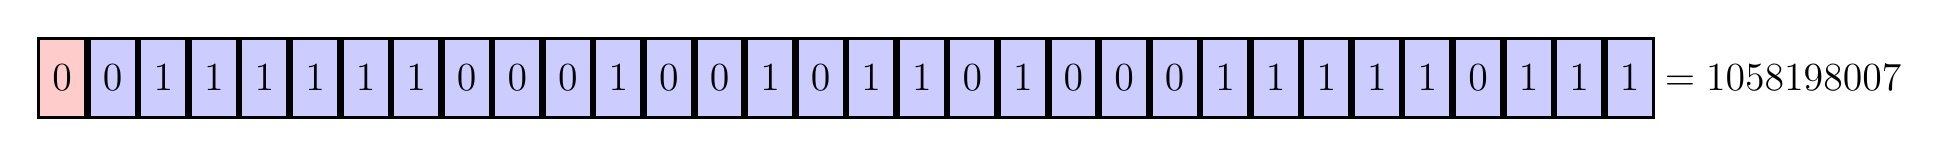
\begin{tikzpicture}

\tikzset{
    box/.style = {
    minimum height=1cm,
    minimum width = 0.6cm
    }
}

\tikzstyle{signe}=[draw, very thick, fill=red!20!white, box]
\tikzstyle{exposant}=[draw, very thick, fill=blue!20!white, box]
\tikzstyle{mantisse}=[draw, very thick, fill=blue!20!white, box]

\matrix [column sep=0cm]
{
\node (f-31) [signe] {\Large 0}; 

& \node (f-30) [exposant] {\Large 0}; 
& \node (f-29) [exposant] {\Large 1}; 
& \node (f-28) [exposant] {\Large 1}; 
& \node (f-27) [exposant] {\Large 1}; 
& \node (f-26) [exposant] {\Large 1}; 
& \node (f-25) [exposant] {\Large 1}; 
& \node (f-24) [exposant] {\Large 1}; 
& \node (f-23) [exposant] {\Large 0}; 

& \node (f-22) [mantisse] {\Large 0}; 
& \node (f-21) [mantisse] {\Large 0}; 
& \node (f-20) [mantisse] {\Large 1}; 
& \node (f-19) [mantisse] {\Large 0}; 
& \node (f-18) [mantisse] {\Large 0}; 
& \node (f-17) [mantisse] {\Large 1}; 
& \node (f-16) [mantisse] {\Large 0}; 
& \node (f-15) [mantisse] {\Large 1};
& \node (f-14) [mantisse] {\Large 1};
& \node (f-13) [mantisse] {\Large 0};
& \node (f-12) [mantisse] {\Large 1};
& \node (f-11) [mantisse] {\Large 0};
& \node (f-10) [mantisse] {\Large 0};
& \node (f-9) [mantisse] {\Large 0};
& \node (f-8) [mantisse] {\Large 1};
& \node (f-7) [mantisse] {\Large 1};
& \node (f-6) [mantisse] {\Large 1};
& \node (f-5) [mantisse] {\Large 1};
& \node (f-4) [mantisse] {\Large 1};
& \node (f-3) [mantisse] {\Large 0};
& \node (f-2) [mantisse] {\Large 1};
& \node (f-1) [mantisse] {\Large 1};
& \node (f-0) [mantisse] {\Large 1};  
\\
};

% \draw ([shift=({0,0.5cm})]f-16.north) node[above] {\Large \emph{Magic number} $0x5F3759DF$};

\draw ([shift=({0,0cm})]f-0.east) node[right] {\Large $= 1058198007$};

\end{tikzpicture}

%%%

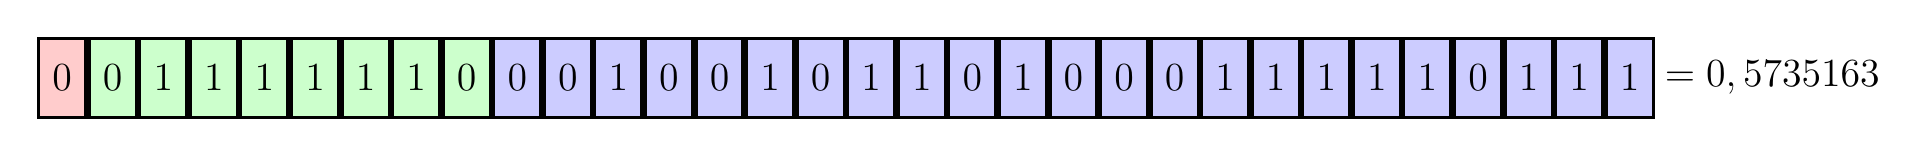
\begin{tikzpicture}

\tikzset{
    box/.style = {
    minimum height=1cm,
    minimum width = 0.6cm
    }
}

\tikzstyle{signe}=[draw, very thick, fill=red!20!white, box]
\tikzstyle{exposant}=[draw, very thick, fill=green!20!white, box]
\tikzstyle{mantisse}=[draw, very thick, fill=blue!20!white, box]

\matrix [column sep=0cm]
{
\node (f-31) [signe] {\Large 0}; 

& \node (f-30) [exposant] {\Large 0}; 
& \node (f-29) [exposant] {\Large 1}; 
& \node (f-28) [exposant] {\Large 1}; 
& \node (f-27) [exposant] {\Large 1}; 
& \node (f-26) [exposant] {\Large 1}; 
& \node (f-25) [exposant] {\Large 1}; 
& \node (f-24) [exposant] {\Large 1}; 
& \node (f-23) [exposant] {\Large 0}; 

& \node (f-22) [mantisse] {\Large 0}; 
& \node (f-21) [mantisse] {\Large 0}; 
& \node (f-20) [mantisse] {\Large 1}; 
& \node (f-19) [mantisse] {\Large 0}; 
& \node (f-18) [mantisse] {\Large 0}; 
& \node (f-17) [mantisse] {\Large 1}; 
& \node (f-16) [mantisse] {\Large 0}; 
& \node (f-15) [mantisse] {\Large 1};
& \node (f-14) [mantisse] {\Large 1};
& \node (f-13) [mantisse] {\Large 0};
& \node (f-12) [mantisse] {\Large 1};
& \node (f-11) [mantisse] {\Large 0};
& \node (f-10) [mantisse] {\Large 0};
& \node (f-9) [mantisse] {\Large 0};
& \node (f-8) [mantisse] {\Large 1};
& \node (f-7) [mantisse] {\Large 1};
& \node (f-6) [mantisse] {\Large 1};
& \node (f-5) [mantisse] {\Large 1};
& \node (f-4) [mantisse] {\Large 1};
& \node (f-3) [mantisse] {\Large 0};
& \node (f-2) [mantisse] {\Large 1};
& \node (f-1) [mantisse] {\Large 1};
& \node (f-0) [mantisse] {\Large 1};  
\\
};

% \draw ([shift=({0,0.5cm})]f-16.north) node[above] {\Large \emph{Magic number} $0x5F3759DF$};

\draw ([shift=({0,0cm})]f-0.east) node[right] {\Large $= 0,5735163$};

\end{tikzpicture}

%%%

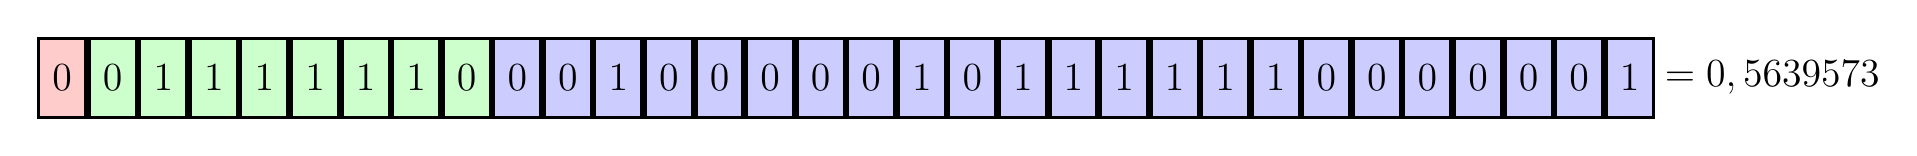
\begin{tikzpicture}

\tikzset{
    box/.style = {
    minimum height=1cm,
    minimum width = 0.6cm
    }
}

\tikzstyle{signe}=[draw, very thick, fill=red!20!white, box]
\tikzstyle{exposant}=[draw, very thick, fill=green!20!white, box]
\tikzstyle{mantisse}=[draw, very thick, fill=blue!20!white, box]

\matrix [column sep=0cm]
{
\node (f-31) [signe] {\Large 0}; 

& \node (f-30) [exposant] {\Large 0}; 
& \node (f-29) [exposant] {\Large 1}; 
& \node (f-28) [exposant] {\Large 1}; 
& \node (f-27) [exposant] {\Large 1}; 
& \node (f-26) [exposant] {\Large 1}; 
& \node (f-25) [exposant] {\Large 1}; 
& \node (f-24) [exposant] {\Large 1}; 
& \node (f-23) [exposant] {\Large 0}; 

& \node (f-22) [mantisse] {\Large 0}; 
& \node (f-21) [mantisse] {\Large 0}; 
& \node (f-20) [mantisse] {\Large 1}; 
& \node (f-19) [mantisse] {\Large 0}; 
& \node (f-18) [mantisse] {\Large 0}; 
& \node (f-17) [mantisse] {\Large 0}; 
& \node (f-16) [mantisse] {\Large 0}; 
& \node (f-15) [mantisse] {\Large 0};
& \node (f-14) [mantisse] {\Large 1};
& \node (f-13) [mantisse] {\Large 0};
& \node (f-12) [mantisse] {\Large 1};
& \node (f-11) [mantisse] {\Large 1};
& \node (f-10) [mantisse] {\Large 1};
& \node (f-9) [mantisse] {\Large 1};
& \node (f-8) [mantisse] {\Large 1};
& \node (f-7) [mantisse] {\Large 1};
& \node (f-6) [mantisse] {\Large 0};
& \node (f-5) [mantisse] {\Large 0};
& \node (f-4) [mantisse] {\Large 0};
& \node (f-3) [mantisse] {\Large 0};
& \node (f-2) [mantisse] {\Large 0};
& \node (f-1) [mantisse] {\Large 0};
& \node (f-0) [mantisse] {\Large 1};  
\\
};

% \draw ([shift=({0,0.5cm})]f-16.north) node[above] {\Large \emph{Magic number} $0x5F3759DF$};

\draw ([shift=({0,0cm})]f-0.east) node[right] {\Large $= 0,5639573$};

\end{tikzpicture}
 
\end{document}